\section{Hallucination and Uncertainty}

\begin{frame}{}
    \LARGE Research Frontiers: \textbf{Hallucination and Uncertainty}

    \vspace{1em}
    \normalsize Why does a model guess, and can it know when it does not know?
\end{frame}

\begin{frame}{A Puzzle: Better Reasoners That Hallucinate More}
    \begin{center}
    \small
    \begin{adjustbox}{max width=\linewidth}\begin{tabular}{lccc}
        \toprule
        \textbf{SimpleQA, no web access} & \textbf{Accuracy} & \textbf{Hallucination rate} & \textbf{Abstains} \\
        \midrule
        o1 (2024) & 0.47 & 0.44 & 0.09 \\
        o3 (Apr 2025) & 0.49 & 0.51 & 0.00 \\
        \rowcolor{KAred!10} o4-mini (Apr 2025) & 0.20 & 0.79 & 0.01 \\
        \rowcolor{KAUSTcyan!12} gpt-5-thinking-mini (Aug 2025) & 0.22 & 0.26 & 0.52 \\
        \bottomrule
    \end{tabular}\end{adjustbox}
    \end{center}
    \begin{itemize}\itemsep0.45em
        \item o3 hallucinates more than o1. OpenAI's reading: it \emph{``tends to make more claims overall''}.
        \item The two small models \textbf{know about the same amount} (0.20 and 0.22). One answers almost everything. The other declines half the time.
        \item So hallucination is not only a knowledge problem. It is a \textbf{decision}: answer, or abstain.
    \end{itemize}
    \vspace{0.2em}
    \caveat{``Hallucination rate'' here is wrong answers over \emph{all} questions. The abstain column is derived as the remainder.}
    \src{OpenAI, ``o3 and o4-mini System Card'' (Apr 2025), Table 4. OpenAI, ``GPT-5 System Card'' (Aug 2025), Table 8. Wei et al., ``Measuring short-form factuality in large language models,'' \href{https://arxiv.org/abs/2411.04368}{arXiv:2411.04368}.}
\end{frame}

\begin{frame}{Two Terms, and a Floor on Error}
    \begin{itemize}\itemsep0.6em
        \item \textbf{Hallucination:} a \emph{plausible falsehood}. \textbf{Confabulation:} an answer that is wrong \emph{and arbitrary}, so it changes with the random seed.
        \item \textbf{A floor on error.} No computable model can learn every computable function, so \emph{some} error is unavoidable for any language model, however large.
        \item \textbf{What the floor does not say:} how much error, on which questions, and whether the model answers or declines. The puzzle on the previous slide lives above this floor.
        \item The useful question therefore becomes: \emph{when} does a model choose to answer?
    \end{itemize}
    \vspace{0.3em}
    \takeaway{Unavoidable error sets a floor. Above it, the hallucination rate depends on what the model was trained and scored to do.}
    \src{Xu, Jain, Kankanhalli, ``Hallucination is Inevitable: An Innate Limitation of Large Language Models,'' \href{https://arxiv.org/abs/2401.11817}{arXiv:2401.11817}. Farquhar et al., Nature 630 (2024).}
\end{frame}

\begin{frame}{What Post-Training Does to Calibration}
    \begin{columns}[T,onlytextwidth]
        \column{0.5\textwidth}
        \centering
        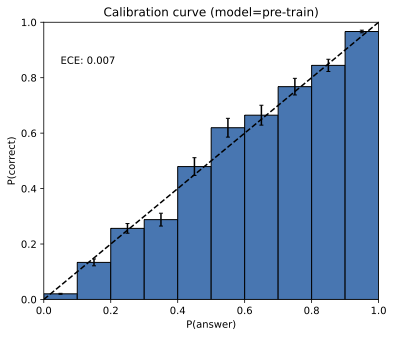
\includegraphics[width=0.49\linewidth,height=0.38\textheight,keepaspectratio]{images/research-frontiers/kalai_fig2_gpt4_calibration_pretrain.png}
        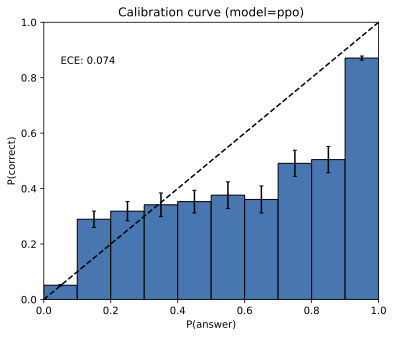
\includegraphics[width=0.49\linewidth,height=0.38\textheight,keepaspectratio]{images/research-frontiers/kalai_fig2_gpt4_calibration_ppo.png}

        {\scriptsize GPT-4 on an MMLU subset. Left: after pre-training, ECE 0.007. Right: after PPO post-training, ECE 0.074.}
        \column{0.48\textwidth}
        \begin{itemize}\itemsep0.4em
            \item \textbf{Pre-training} gives a calibrated model. \textbf{RLHF} worsens calibration tenfold.
            \item \textbf{Reasoning fine-tuning lowers abstention by 24\%} on average on unanswerable questions. Scale has almost no effect.
        \end{itemize}
    \end{columns}
    \vspace{0.3em}
    \takeaway{Every stage after pre-training optimises a score that pays for answers. None of them pays for saying ``I don't know''.}
    \src{Figures: Kalai et al., \href{https://arxiv.org/abs/2509.04664}{arXiv:2509.04664}, Figure 2, from OpenAI, ``GPT-4 Technical Report,'' Figure 8. Kirichenko, Ibrahim, Chaudhuri, Bell, ``AbstentionBench,'' \href{https://arxiv.org/abs/2506.09038}{arXiv:2506.09038}.}
\end{frame}

\begin{frame}{Uncertainty Estimation: a Ladder of Cost and Access}
    \begin{center}
    \small
    \renewcommand{\arraystretch}{1.15}
    \begin{adjustbox}{max width=\linewidth}\begin{tabular}{>{\raggedright\arraybackslash}p{3.5cm}>{\raggedright\arraybackslash}p{2.8cm}>{\raggedright\arraybackslash}p{2.0cm}>{\raggedright\arraybackslash}p{3.7cm}}
        \toprule
        \textbf{Method} & \textbf{Cost} & \textbf{Access} & \textbf{Weakness} \\
        \midrule
        Token log-probability, entropy & 1 pass & logits & paraphrases look like doubt \\
        Semantic entropy probe & 1 pass + linear probe & hidden states & white-box only \\
        Verbalised confidence & 1 pass & black box & consistently overconfident \\
        P(True) & 1 to 2 passes & logits & needs the right format \\
        \rowcolor{KAUSTcyan!12} Semantic entropy & 5 to 10 samples + NLI & black box & blind to systematic errors \\
        Conformal wrapper & wraps any score & any & needs labelled data \\
        \bottomrule
    \end{tabular}\end{adjustbox}
    \end{center}
    \begin{itemize}\itemsep0.4em
        \item Nothing wins everywhere. The first question is not ``which is best?'' but ``what can I afford, and what can I see?''
    \end{itemize}
    \src{Farquhar, Kossen, Kuhn, Gal, Nature 630 (2024). Kossen et al., \href{https://arxiv.org/abs/2406.15927}{arXiv:2406.15927}. Xiong et al., \href{https://arxiv.org/abs/2306.13063}{arXiv:2306.13063}. Kadavath et al., \href{https://arxiv.org/abs/2207.05221}{arXiv:2207.05221}. Shelmanov et al., ACL 2025 tutorial on uncertainty quantification.}
\end{frame}

\begin{frame}{Acting on Uncertainty: Guarantee, Abstain, Verify}
    \begin{center}
    \small
    \renewcommand{\arraystretch}{1.15}
    \begin{adjustbox}{max width=\linewidth}\begin{tabular}{>{\raggedright\arraybackslash}p{2.9cm}>{\raggedright\arraybackslash}p{5.3cm}>{\raggedright\arraybackslash}p{4.4cm}}
        \toprule
        \textbf{Approach} & \textbf{How} & \textbf{Reported effect} \\
        \midrule
        Conformal factuality & drop the least supported sub-claims until a calibrated threshold is met & 80 to 90\% correctness guarantees \\
        R-Tuning & fine-tune on data labelled with what the model does not know & refuses 87 to 99\% of unanswerable questions \\
        Abstention-aware RL & reward declining when likely wrong & up to 10.3 points of precision (one 2026 preprint) \\
        \bottomrule
    \end{tabular}\end{adjustbox}
    \end{center}
    \begin{itemize}\itemsep0.4em
        \item The trend follows the diagnosis: from refusal data and filtering (2023 to 2024) to \textbf{rewards that pay for abstention} (2026).
        \item \textbf{The open trade-off:} precision against coverage. Abstaining on everything is trivially safe.
        \item \textbf{Not settled.} A formal result says wrong definite answers cannot be removed entirely, so the real quantity is \emph{coverage} at guaranteed correctness.
    \end{itemize}
    \src{Mohri, Hashimoto, \href{https://arxiv.org/abs/2402.10978}{arXiv:2402.10978}. Zhang, Diao et al., ``R-Tuning,'' \href{https://arxiv.org/abs/2311.09677}{arXiv:2311.09677}, Table 3. Zhang et al., ``AWA-RL,'' \href{https://arxiv.org/abs/2607.10738}{arXiv:2607.10738}. Imamura, ``Hallucination, abstention, and computable inseparability,'' \href{https://arxiv.org/abs/2604.28067}{arXiv:2604.28067}.}
\end{frame}

\begin{frame}{Measuring It in 2026: the Metric Keeps Moving}
    \begin{columns}[T,onlytextwidth]
        \column{0.47\textwidth}
        \centering
        \small
        \renewcommand{\arraystretch}{1.15}
        \begin{adjustbox}{max width=\linewidth}\begin{tabular}{lc}
            \toprule
            \textbf{AA-Omniscience, 3 Oct 2026} & \textbf{Index} \\
            \midrule
            Claude Opus 5.5 (Max) & 46 \\
            GPT-6 Astra (High) & 44 \\
            Claude Fable 5.1 (Max) & 43 \\
            Best model at release, Nov 2025 & 4.8 \\
            \bottomrule
        \end{tabular}\end{adjustbox}

        \vspace{0.4em}
        {\scriptsize Index from $-100$ to 100. Correct answers add, hallucinations subtract, abstentions count zero.}
        \column{0.51\textwidth}
        \begin{itemize}\itemsep0.4em
            \item \textbf{Scoring now penalises wrong answers}, so a guess no longer beats an abstention.
            \item \textbf{Low hallucination is not knowledge.} The lowest rate on the board, 1\%, belongs to a 1B model.
            \item \textbf{First-party reports diverge.} Anthropic reports a net score. OpenAI's Astra card gives no SimpleQA or abstention numbers. Google's September cards give no factuality metric.
            \item \textbf{Judges are in the loop.} Graders agree with humans 72 to 75\% of the time.
        \end{itemize}
    \end{columns}
    \vspace{0.2em}
    \src{Jackson et al., ``AA-Omniscience,'' \href{https://arxiv.org/abs/2511.13029}{arXiv:2511.13029}, and live leaderboard (opened 2026-10-03). Anthropic, ``Claude Opus 5.5 System Card.'' OpenAI, ``GPT-6 Astra System Card'' and ``GPT-5 System Card.'' Wei et al., \href{https://arxiv.org/abs/2403.18802}{arXiv:2403.18802}.}
\end{frame}

\begin{frame}{Hallucination: What to Remember}
    \begin{itemize}\itemsep0.55em
        \item Some error is \textbf{unavoidable in principle}. Above that floor, hallucination is partly \textbf{a decision}: answer or abstain.
        \item \textbf{Post-training makes it worse}: RLHF degrades calibration, and reasoning fine-tuning lowers abstention.
        \item \textbf{Uncertainty estimators} trade cost against access. None wins everywhere.
        \item The fixes that match the diagnosis are \textbf{abstention-aware scoring and rewards}, judged by coverage at guaranteed correctness.
        \item Read a hallucination rate \textbf{together with accuracy and abstention}.
    \end{itemize}
    \vspace{0.4em}
    \takeaway{\textbf{Next.} Some 2026 preprints suggest the model \emph{has} the uncertainty signal inside and does not act on it. To check a claim like that, we have to look inside.}
\end{frame}
